
\chapter{Introducción al modelo Estándar}

La física de partículas estudia los constituyentes universales del universo, esto es, las \textit{partículas elementales}, así como las interacciones entre estas. En la actualidad el modelo estándar es la teoría que mejor describe el comportamiento de estas partículas. Las partículas elementales descritas en el modelo se recogen en la siguiente imagen:

\begin{figure}[h!] \centering
	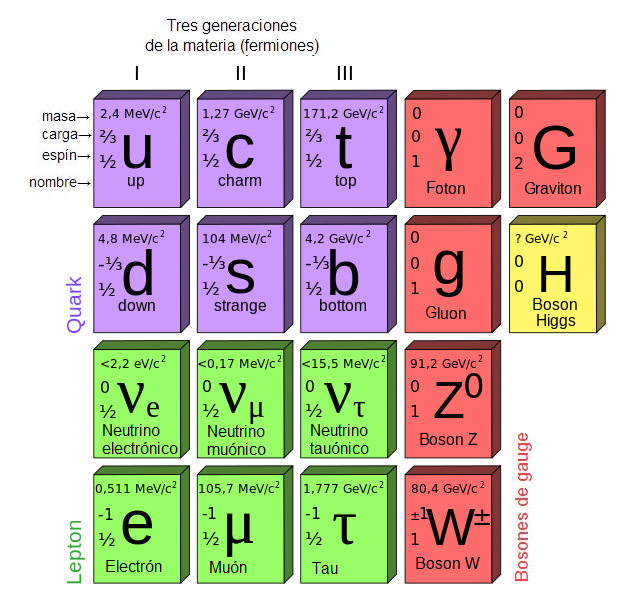
\includegraphics[width=0.65\textwidth]{Cuerpo/Ch_00/1_01_Modelo_Estandar.png}
	\caption{Partículas fundamentales según el modelo estándar}
\end{figure}
La dinámica de los doce fermiones está descrita por la Ecuación de Dirac, que se encuentra dentro de la Mecánica Cuántica Relativista

\newpage

Hola 